\documentclass[a4paper, 12 pt]{article}

\usepackage[x11names]{xcolor}
\usepackage[top=0.75in, bottom=0.2in, left=0.35in, right=0.35in]{geometry}
\usepackage{graphicx}
\usepackage{booktabs}
\usepackage{url}
\usepackage{enumitem}
\usepackage{palatino}
\usepackage{tabularx}

\newcommand{\coloredSectionDark}[1]{{\small \colorbox{DodgerBlue2}{\begin{minipage}{0.99\textwidth}{\textbf{#1 \vphantom{p\^{E}}}}\end{minipage}}}}
\newcommand{\coloredSection}[1]{{\small \colorbox{DeepSkyBlue1}{\begin{minipage}{0.99\textwidth}{\textbf{#1 \vphantom{p\^{E}}}}\end{minipage}}}}

\begin{document}
\section*{\textcolor{DodgerBlue2}{APRILPROJEKT - KUCHEN BACKEN}}

\noindent
\coloredSectionDark{\textbf{\textcolor{white}{FAZIT}}}\\[-0.3cm]
\\\\
Alle Schritte sind voneinander abhängig und für das optimale gelingen darf die Reihenfolge nicht vertauscht werden.

\begin{figure}[h!]
    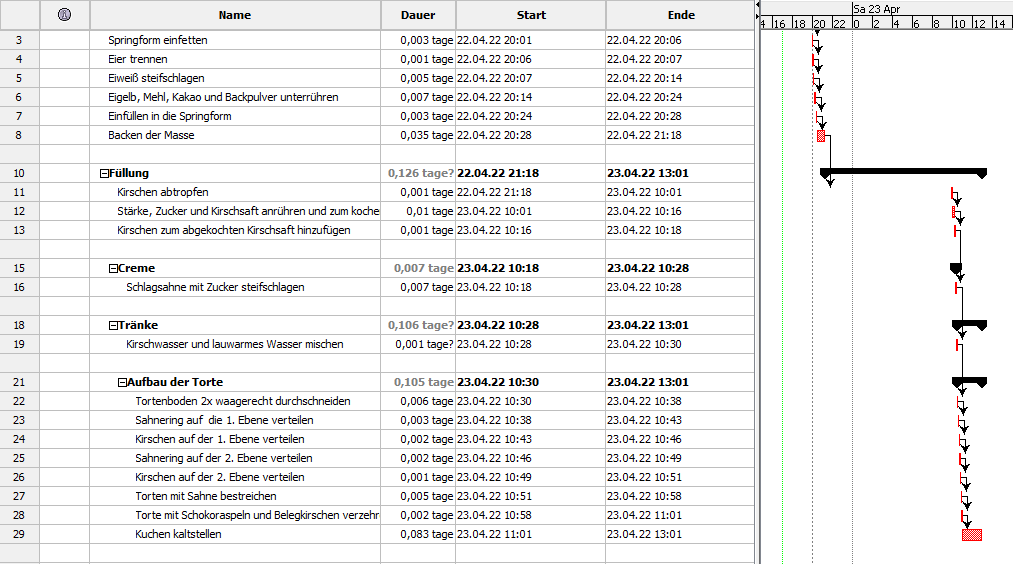
\includegraphics[width=1\linewidth]{timeplan.png}
  \end{figure}
\end{document}